\documentclass[12pt, a4paper, oneside]{report}

%% Encoding & fonts
\usepackage[T1]{fontenc}
\usepackage[utf8]{inputenc}
\usepackage{lmodern}
\usepackage{microtype}

%% Page layout
\usepackage[
  top=3cm, bottom=3cm,
  left=3.5cm, right=2.5cm,
  headheight=15pt
]{geometry}
\usepackage{setspace}
\onehalfspacing

%% Headers & footers
\usepackage{fancyhdr}

%% Mathematics
\usepackage{amsmath, amssymb, amsthm}

%% Figures & tables
\usepackage{graphicx}
\graphicspath{{figures/}}
\usepackage{booktabs}
\usepackage{caption}
\usepackage{subcaption}
\usepackage{float}

%% Listings (code)
\usepackage{listings}
\usepackage{xcolor}

%% Hyperlinks
\usepackage[hidelinks]{hyperref}
\usepackage{cleveref}

%% Bibliography (BibLaTeX + biber)
\usepackage[
  backend=biber,
  style=authoryear,
  sorting=nyt,
  natbib=true
]{biblatex}
\addbibresource{references.bib}

\begin{document}

The tip of a single vector with constant magnitude and a variable angle will trace out a circle.

\begin{figure}[H]
  \centering
  \begin{subfigure}[b]{0.3\textwidth}
    
\includegraphics[width=\textwidth]{single-vector-animation/1}
  \end{subfigure}
  \hfill
  \begin{subfigure}[b]{0.3\textwidth}
    
\includegraphics[width=\textwidth]{single-vector-animation/2}
  \end{subfigure}
  \hfill
  \begin{subfigure}[b]{0.3\textwidth}
    
\includegraphics[width=\textwidth]{single-vector-animation/3}
  \end{subfigure}
  \caption{\href{https://github.com/matia128/thesis/blob/master/figures/single-vector-animation/single-vector-animation.gif}{View animation}}
  \label{fig:single-vector-animation}
\end{figure}

When a pair of vectors with magnitudes $a$ and $b$ and variable angles $\theta$ and $\phi$ are allowed to rotate at constant rates, they will produce a curve known as a centered trochoid traced by the tip of their resultant, $P$.

\begin{figure}[H]
  \centering
  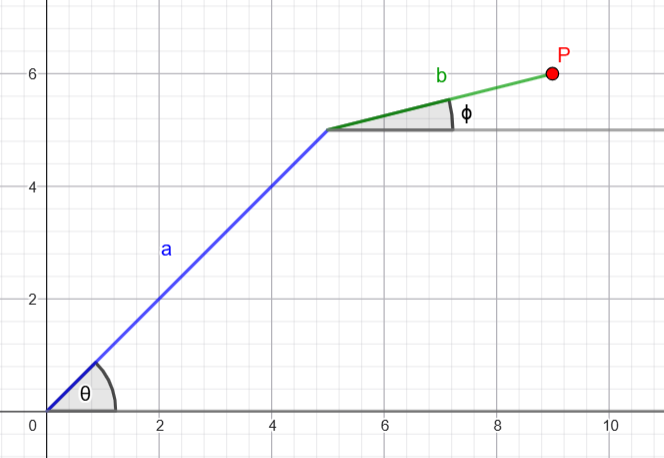
\includegraphics[width=0.7\textwidth]{two-vector-diagram-with-initial-labels}
  \caption{}
  \label{fig:two-vector-diagram}
\end{figure}

\begin{figure}[H]
  \centering
  \begin{subfigure}[b]{0.3\textwidth}
    
\includegraphics[width=\textwidth]{two-vector-animation/1}
  \end{subfigure}
  \hfill
  \begin{subfigure}[b]{0.3\textwidth}
    
\includegraphics[width=\textwidth]{two-vector-animation/2}
  \end{subfigure}
  \hfill
  \begin{subfigure}[b]{0.3\textwidth}
    
\includegraphics[width=\textwidth]{two-vector-animation/3}
  \end{subfigure}
  \caption{\href{https://github.com/matia128/thesis/blob/master/figures/two-vector-animation/two-vector-animation.gif}{View animation}}
  \label{fig:two-vector-animation}
\end{figure}

The shape traced by the vectors is dictated by the ratios of $a$ to $b$ and $\theta$ to $\phi$. We can set $a$ to 1 and $\rho$ to $b/a$ while setting $f$ to $\phi/\theta$ and substituting $\phi$ with $f\theta$.
This manipulation of variables preserves the shape of the curve while discarding its size and the duration of its construction.

\begin{figure}[H]
  \centering
  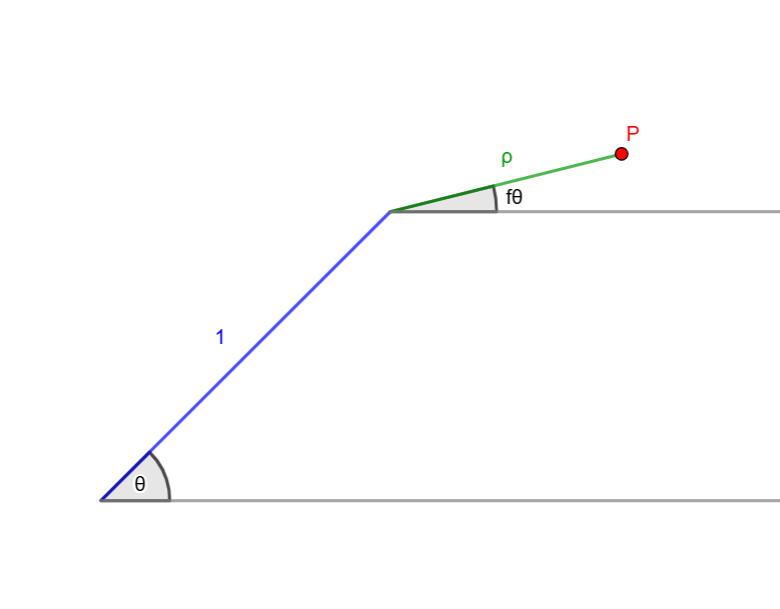
\includegraphics[width=0.7\textwidth]{two-vector-diagram-with-updated-labels}
  \caption{}
  \label{fig:two-vector-diagram-updated}
\end{figure}

Each shape is now identified with only two parameters, $\rho$ and $f$, which represent the ratio of magnitudes and the ratio of angular frequencies respectively.

When converted to Cartesian coordinates, the vectors become $(\cos\theta, \sin\theta)$ and $(\rho\cos f\theta, \rho\sin f\theta)$.
The tracing point, $P$, is given by the sum of the two vectors:

\begin{equation}
(\cos\theta + \rho\cos f\theta, \sin\theta + \rho\sin f\theta).
\end{equation}

\newpage

In the complex plane, these coordinates can be represented by the complex number:
\begin{equation*}
z = x + iy
\end{equation*}

Substituting:
\begin{equation*}
z(\theta) = (\cos\theta + \rho\cos f\theta) + i(\sin\theta + \rho\sin f\theta)
\end{equation*}

Rearranging:

\begin{equation*}
z(\theta) = \cos\theta + i\sin\theta + \rho\cos f\theta + i\rho\sin f\theta
\end{equation*}

Applying Euler's formula:
\begin{equation}
z(\theta) = e^{i\theta} + \rho e^{if\theta}
\end{equation}

A few examples are given below:

\begin{figure}[H]
  \centering
  \begin{subfigure}[b]{0.3\textwidth}
    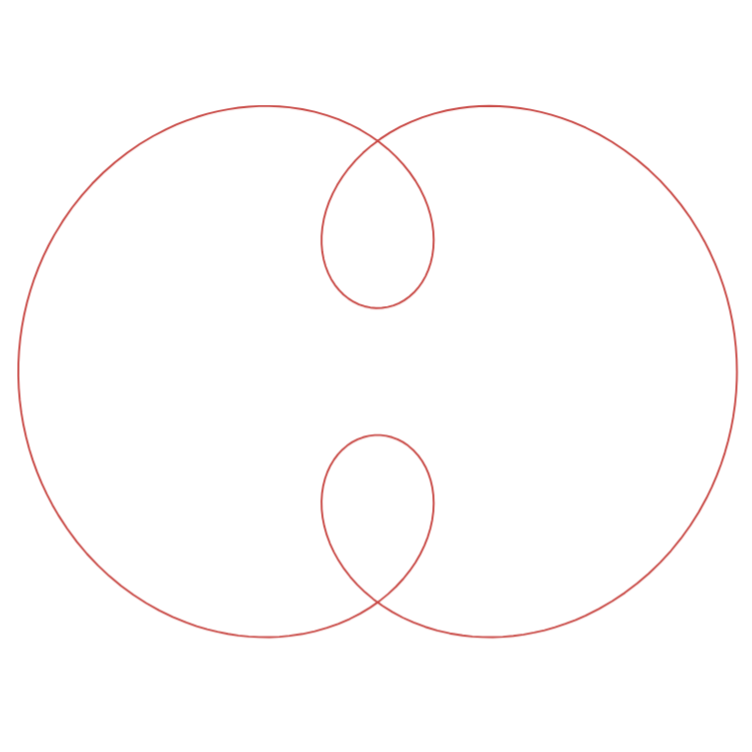
\includegraphics[width=\textwidth]{centered-trochoids-gallery/1}
  \end{subfigure}
  \hfill
  \begin{subfigure}[b]{0.3\textwidth}
    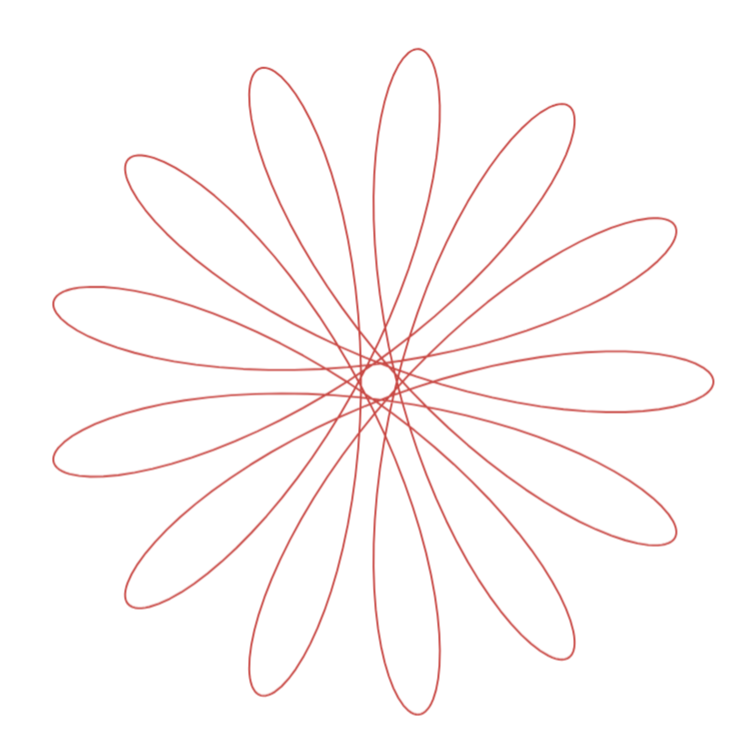
\includegraphics[width=\textwidth]{centered-trochoids-gallery/2}
  \end{subfigure}
  \hfill
  \begin{subfigure}[b]{0.3\textwidth}
    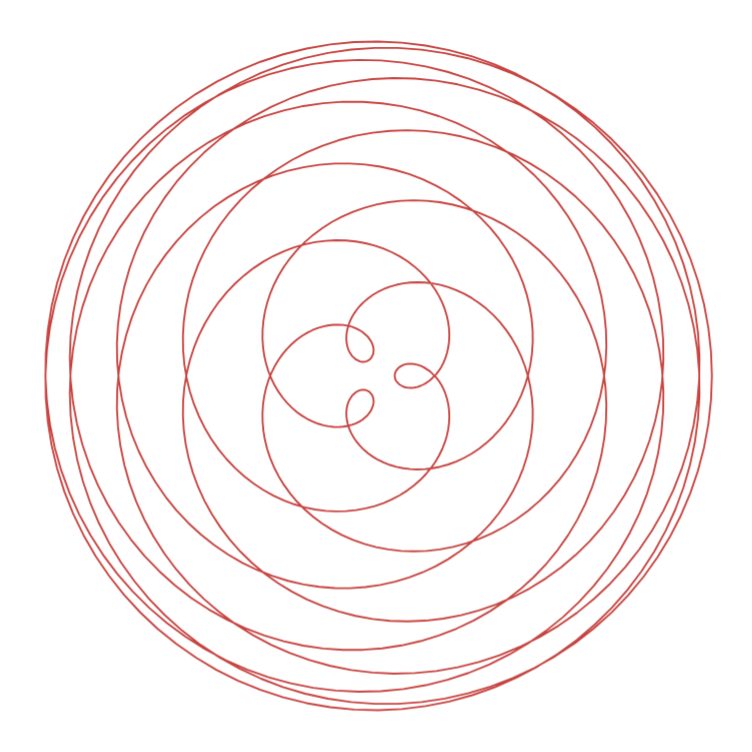
\includegraphics[width=\textwidth]{centered-trochoids-gallery/3}
  \end{subfigure}

  \vspace{0.5em}

  \begin{subfigure}[b]{0.3\textwidth}
    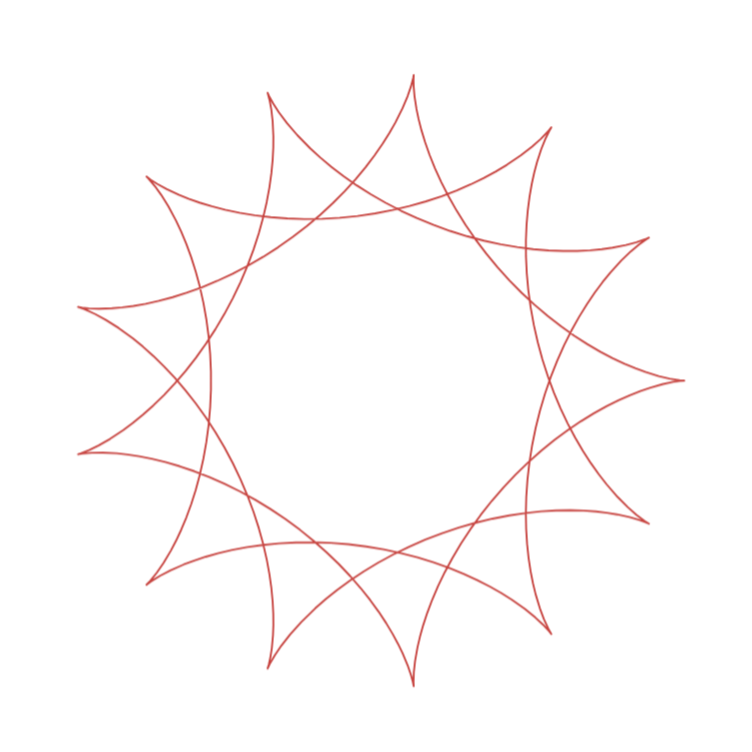
\includegraphics[width=\textwidth]{centered-trochoids-gallery/4}
  \end{subfigure}
  \hfill
  \begin{subfigure}[b]{0.3\textwidth}
    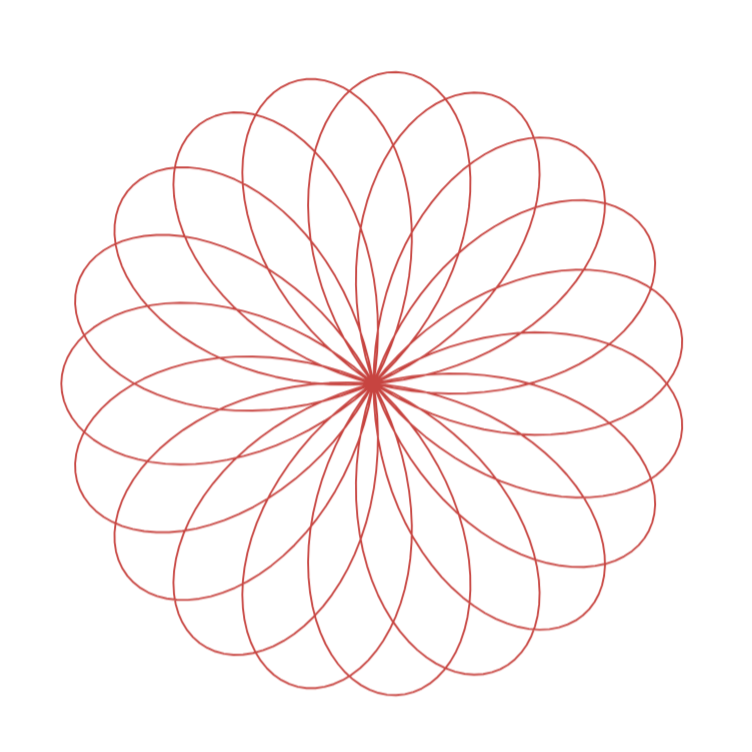
\includegraphics[width=\textwidth]{centered-trochoids-gallery/5}
  \end{subfigure}
  \hfill
  \begin{subfigure}[b]{0.3\textwidth}
    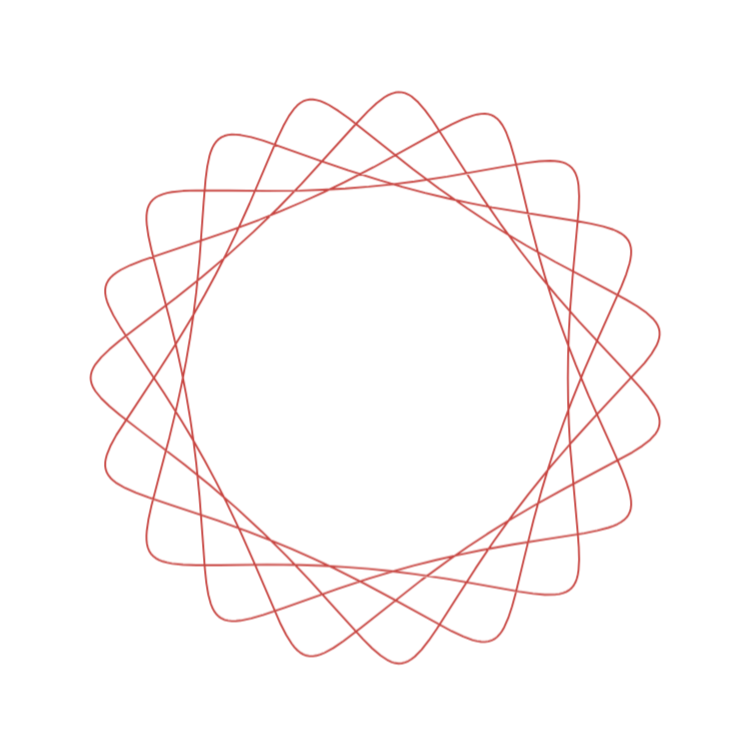
\includegraphics[width=\textwidth]{centered-trochoids-gallery/6}
  \end{subfigure}
  \caption{\href{https://www.desmos.com/calculator/7msxvmmdxj}{Interactive Desmos graph}}
  \label{fig:gallery}
\end{figure}

\end{document}
